\begin{comment} -Insert citations.  -Fix chalmers univ of tech ref in line 16
\end{comment}

In this chapter we present the results of our experiments that we performed to
evaluate the correctness and performance of our compiler. We demonstrate the
effects on performance due to the differnt approaches to compile arrays, and due
to togglingi of various compilation switches. We also compare our results to
those of other \matlab compilers including the de facto Mathworks' compiler,
\matlab coder (also provided by Mathworks)~\cite{}, and the \mctwofor~\cite{}
compiler. 

The set of benchmarks used for our experiments consists of benchmarks from
various sources; Most of them are from related projects like FALCON~\cite{} and
OTTER~\cite{}, Chalmers university of Technology~\cite{}, ``Mathworks' central
file excahnge''~\cite{}, and the presentation on parallel programming in \matlab
by Burkardt and Cliff~\cite{}. 

Below is a brief description of each benchmark that we used: \begin{itemize}
\item \emph{bbai} is an implementation of the Babai estimation algorithm and
consists of random number generation and operations on a 2-dimensional array in
a loop.  \item \emph{bubl} is the standard bubble sort algorithm. It is
characterized by nested loops and read/write operations on a large row vector.
\item \emph{capr} computes the capacitance of a transmission line using finite
difference and Gauss-Seidel method. It involves loop-based operations on two
2-dimensional arrays.  \item \emph{clos} calculates the transitive closure of a
directed graph. Its key feature is matrix multiplication operation on two large
2-dimensional arrays.  \item \emph{crni} computes the Crank-Nicholson solution
to the heat equation.  This benchmark involves some elementary scalar operations
on a very large (2300$\times$2300) array.  \item \emph{dich} computes Dirichlet
solution to Laplace's equation. It involves loop-based operation on a
2-dimensional array.  \item \emph{diff} calculates diffraction pattern of
monochromatic light. Its key feature is explicit array growth via concatenation
operation.  \item \emph{edit} calculates the edit distance between two strings.
It involves operations on large row vectors of \texttt{chars}.  \item
\emph{fiff} computes the finite difference solution to the wave equation.  It
also involves loop-based operations on a 2-dimensional array.  \item \emph{lgdr}
calculates derivatives of Legendre polynomials. It is characterized by transpose
operation on row vectors.  \item \emph{mbrt} computes Mandelbrot sets. It
involves operations on scalar data of \texttt{complex} type. It also involves
\texttt{parfor} loop.  \item \emph{nb1d} simulates the 1-dimensional n-body
problem. It involves operations on column vectors in nested loops including a
\texttt{parfor} loop.  \item \emph{matmul} implements the naive matrix
multiplication. It involves three nested loops including one \texttt{parfor}
loop, and read/write operations on three large 2-dimensional arrays.  \item
\emph{mcpi} calculates the value of $\pi$ using the Monte carlo algorithm.  It
involves random number generation in a loop. It also uses \texttt{parfor} loop.
\item \emph{numprime} calculates the number of prime numbers upto a given value
using the sieve of eratosthenes. It features a \texttt{parfor} loop and simple
scalar operations.  \item \emph{optstop} solves the optimal stopping problem. It
involves operations on a row vector, random number generation and a
\texttt{parfor} loop.  \item \emph{quadrature} simulates the quadrature approach
to calculate integral of a function. It involves scalar values and a
\texttt{parfor} loop.  \end{itemize}

We used \matlab release R2013a to execute our benchmarks in \matlab and \matlab
coder. We also executed them using the GNU Octave version 3.2.4. We compiled our
benchmarks to Fortran using the \mctwofor compiler and compiled the generated
Fortran code using the GCC 4.6.3 GFortran compiler with optimization level
\texttt{-O3}. To compile the generated \xten code from our \mixten compiler, we
used \xten version 2.4.0. We used OpenJDK Java 1.7.0\_51 to compile and run Java
code generated by the \xten compiler, and GCC 4.6.4 g++ compiler to compile the
C++ code generated by the \xten compiler. All the experiments were run on a
machine with Intel(R) Core(TM) i7-3820 CPU @ 3.60GHz processor and 16 GB memory
running GNU/Linux(3.8.0-35-generic \#52-Ubuntu). For each benchmark, we used an
input size to make the program run for approximately 20 seconds on the de facto
\matlab compiler. We used the same input sizes for compiling and running
benchmarks via other compilers. We collected the execution times (averaged over
five runs) for each benchmark and compared their speedups over \matlab runtimes
(normalized to one). We summarize our results in the following sections:


\section{\mixten performance comparison with \matlab, \matlab coder, \mctwofor,
and Octave}

We compared the performance of the generated \xten code with that of the
original \matlab code run on Mathworks' implementation of \matlab, and Octave.
We also compared it to the generated C code and Fortran code by \matlab coder
and \mctwofor compilers respectively. 

\begin{figure}[htbp] \begin{center}
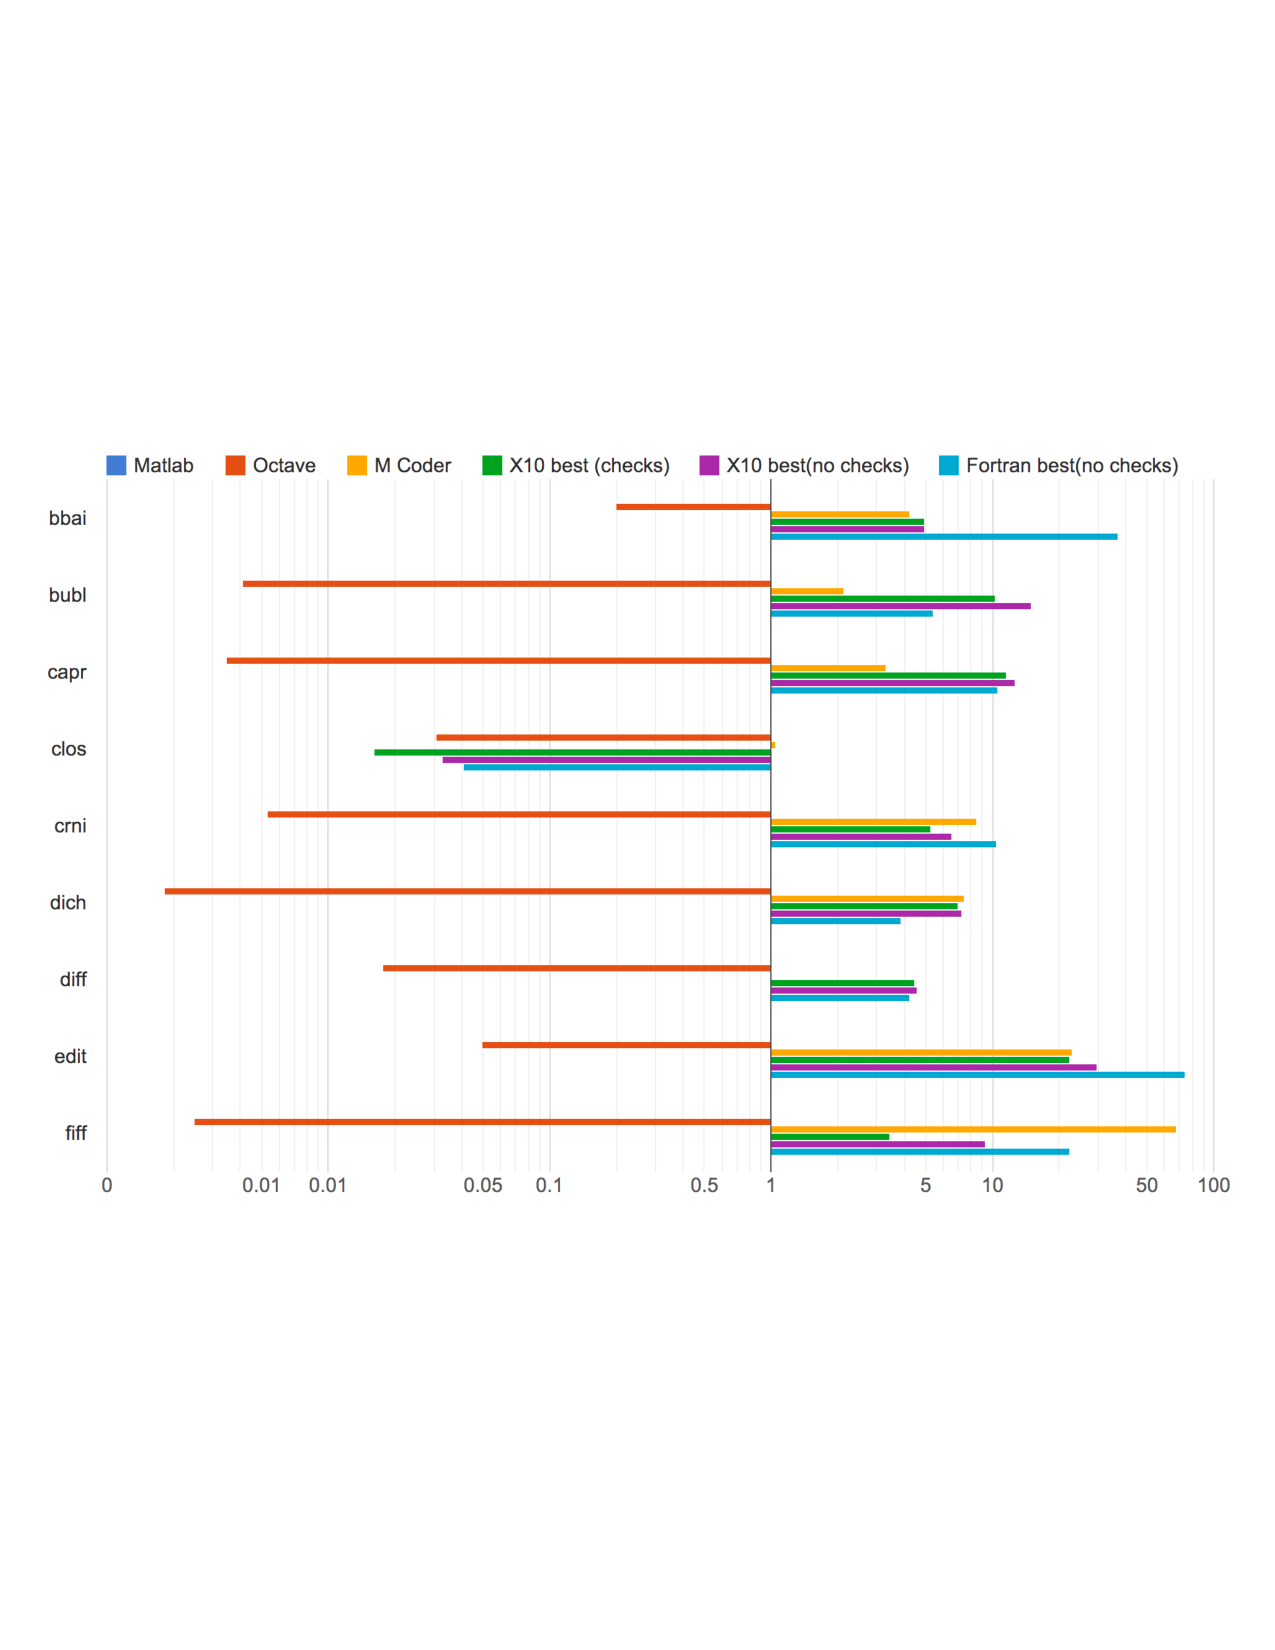
\includegraphics[width=\linewidth]{Figures/final/graph_1_1_1.pdf} \caption
{MiX10 performance comparison (part1) }\label{Fig:graph1_1_1} \end{center}
\end{figure} 
     
\begin{figure}[htbp] \begin{center}
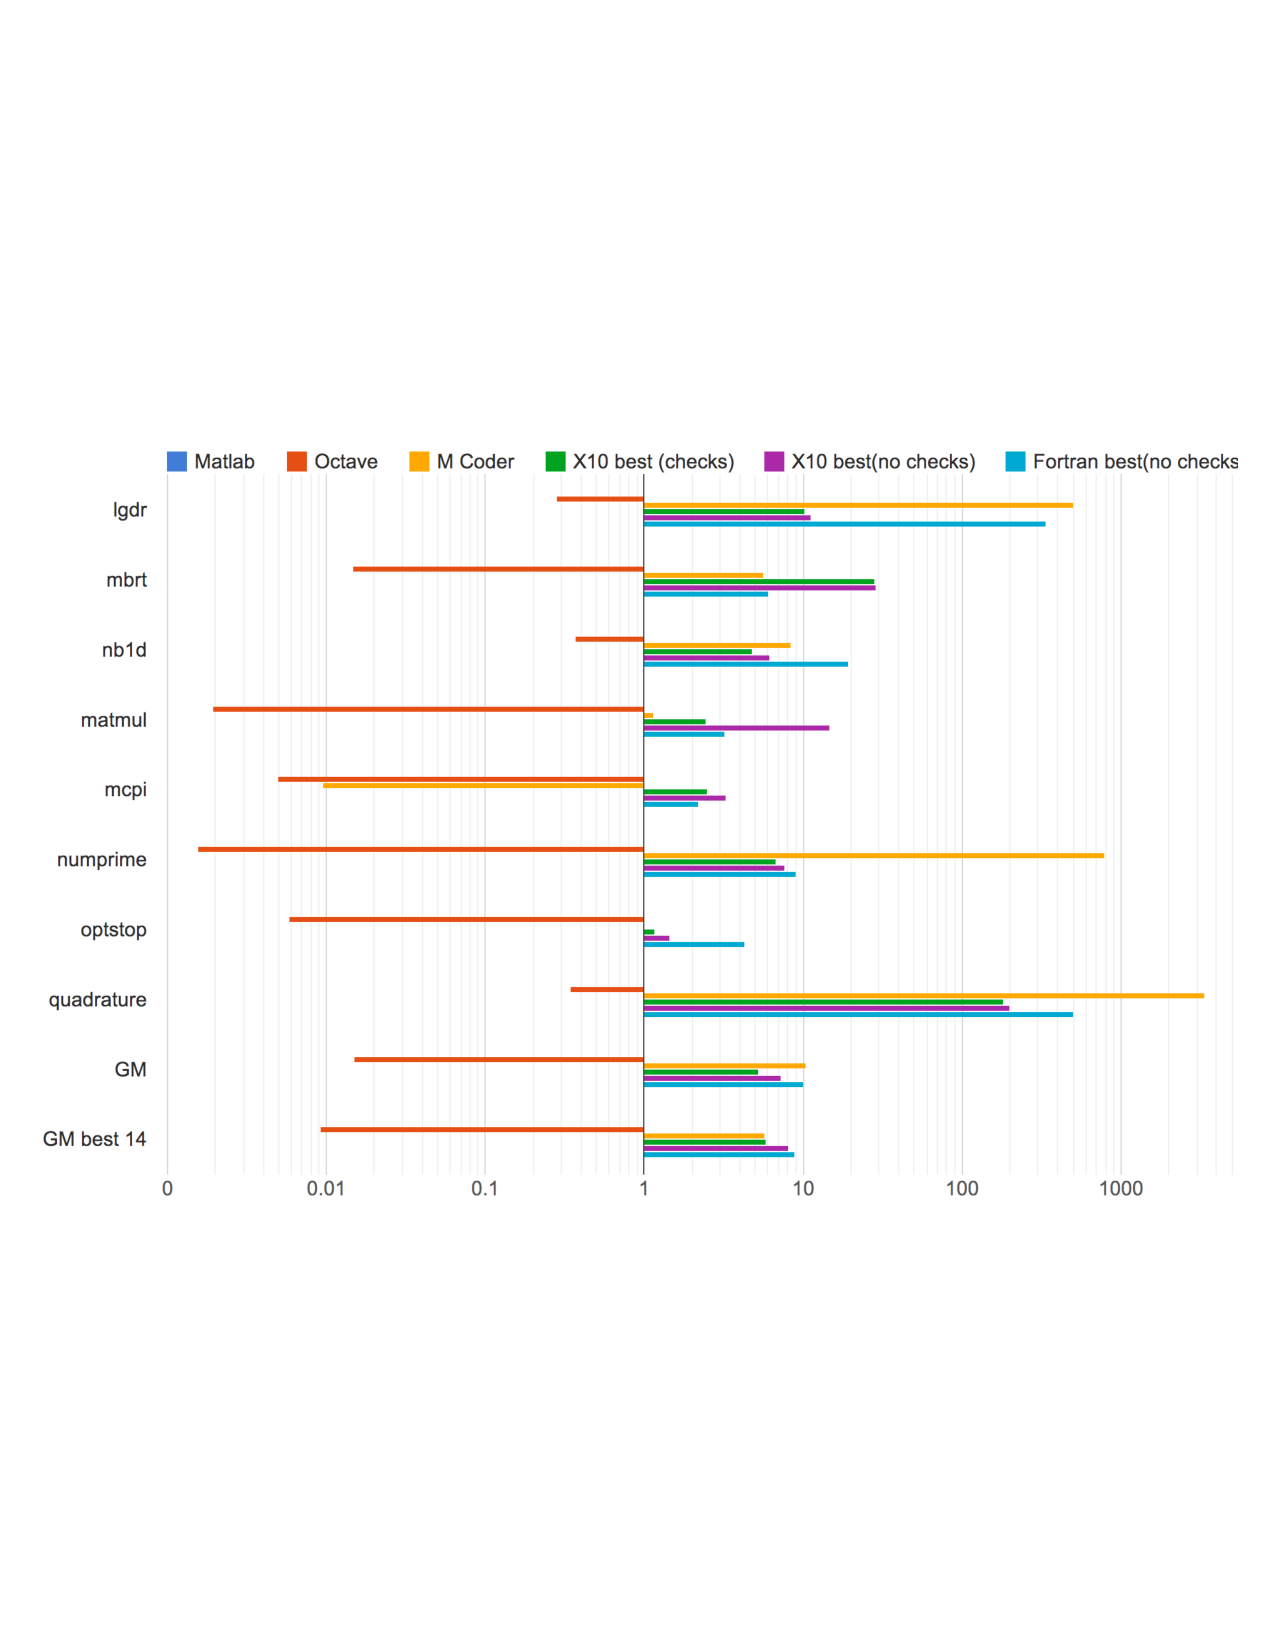
\includegraphics[width=\linewidth]{Figures/final/graph_1_1_2.pdf} \caption
{MiX10 performance comparison (part2) }\label{Fig:graph1_1_2} \end{center}
\end{figure} 

Figures \figref{Fig:graph1_1_1} and \figref{Fig:graph1_1_2} show the speedups
and slowdowns for codes generated for our benchmarks by different compilers.
For \mixten we have included results for generated \xten code by the
\emph{x10c++} compiler with 1) Array bounds checks turned off; and 2) Array
bounds checks turned on. We used the default optimization provided by the \xten
compiler (\texttt{-O}). For Fortran we included the code generated without
bounds checks. C code from \matlab coder was generated with default settings and
includes bounds checks. \figref{Fig:graph1_1_2} also shows the geometric mean of
speedups for all the benchmarks and for our best 14 out of 17 results (compared
to results from \matlab coder). 

We achieved a mean speedup of 5.2 and 7.2 for x10c++ with bounds checks and
x10c++ with no bounds checks respectively.  On the other hand \matlab coder gave
a mean speedup of 10.5 and \mctwofor gave a mean speedup of 10.2. However, we
see that if we do not consider only three benchmarks for which \xten does not
perform as well as C and Fortran, we get a mean sppedup of 5.75 for x10 with
bounds checks compared to 5.72 for C. For no bounds checks we get a mean speedup
of 8.1 compared to 8.8 for Fortran.  We outperform \matlab coder in 8 out of 17
benchmarks, and Fortran in 7 out of 17 benchmarks

\emph{clos} involves builtin matrix
multiplication operations for 2-dimensional matrices. The generated C code from
\matlab coder uses highly optimized matrix multiplication libraries compared to
the naive matrix multiplication implementation used by \mixten. Thus, we get a
speedup of 0.016 as compared to 1.049 for C. Note that the generated Fortran
code is also slowed down (speedup of 0.041) due to the same reason.        

\emph{lgdr} involves repeated transpose of a row vector to a column vector.
\matlab and Fortran, both being array languages are highly optimized for
transpose operations. \mixten currently uses a naive transpose algorithm which
is not as highly optimized. However, we still achieved a speedup of over 10 
times. 

\emph{quadrature} solves the stadard quadrature formula for numerical
integration~\cite{}, which involves repeated arithmetic calculations on a range
of numbers. We achieve a speedup of about 200 times compared to \matlab however
it is slow compared to speedups of 3348 and 502 by C and Fortran respectively.
We believe that \matlab coder leverages partial evaluation for optimizing
numerical methods' implementations.

Other interesting numbers are shown by \emph{optstop}, \emph{numprime} and
\emph{fiff}.
\emph{optstop} involves repeated array indexing by an index of type
\texttt{Double} which needs to be explicitly cast to \texttt{Long}, whenever
used as an index. IntegerOkay analysis cannot convert it to an integer type
because it's the value returned from a call to the \texttt{floor()} function
whose return type is \texttt{Double}. \emph{numprime} involves similar problem,
where the result of the \texttt{sqrt()} function needs to be converted to
\texttt{Long} from \texttt{Double}. \emph{numprime} also involves a for loop
over a conditional that evaluates to true only once. \matlab coder leverages
this fact for optimizing the for loop by implicitly inserting a \texttt{break}
when the conditional becomes true. We tested our generated \xten code by
explicitly inserting a \texttt{break} statement and achieved a speedup of around
65 times. Note that \emph{numprime} is also used for demonstrating
\texttt{parfor} which does not allow a \texttt{break} statement in the loop.
\emph{fiff} is characterized by stencil operations in a loop,
 on a 2-dimensional array. These operations are also optimized by array-based
languages like Fortran and \matlab.  
Note that for \emph{nb1d}, Fortran performs better due to the use of column
vectors in the benchmark, which are represented as 2-dimensional arrays in \xten
but in Fortran they are represented as 1-dimensional and are optimized.

For most of the other benchmarks, we perform better or nearly equal to C and
Fortran code. Inspite of the facts that 1) The sequential core of \xten is a
very high-level object oriented language which is not specialized for
array-based operations; and 2) Generating the executable binaries via \mixten
involves two levels of source-to-source compilations (\matlab $\rightarrow$
\xten $\rightarrow$ C++); We have achieved performance comparable to C and
Fortran.  
       

